% How far a translation gets, by complexity bucket - the three runs of the replicate series.
% Generated by evaluation/figures/pipeline_funnel.py - do not edit by hand.
% Bars are means over the runs; whiskers span the lowest and highest run.
%
% Requires, in the document preamble:
%   \usepackage{pgfplots}
%   \pgfplotsset{compat=1.18}
%
% Then: % How far a translation gets, by complexity bucket - the three runs of the replicate series.
% Generated by evaluation/figures/pipeline_funnel.py - do not edit by hand.
% Bars are means over the runs; whiskers span the lowest and highest run.
%
% Requires, in the document preamble:
%   \usepackage{pgfplots}
%   \pgfplotsset{compat=1.18}
%
% Then: % How far a translation gets, by complexity bucket - the three runs of the replicate series.
% Generated by evaluation/figures/pipeline_funnel.py - do not edit by hand.
% Bars are means over the runs; whiskers span the lowest and highest run.
%
% Requires, in the document preamble:
%   \usepackage{pgfplots}
%   \pgfplotsset{compat=1.18}
%
% Then: % How far a translation gets, by complexity bucket - the three runs of the replicate series.
% Generated by evaluation/figures/pipeline_funnel.py - do not edit by hand.
% Bars are means over the runs; whiskers span the lowest and highest run.
%
% Requires, in the document preamble:
%   \usepackage{pgfplots}
%   \pgfplotsset{compat=1.18}
%
% Then: \input{figures/pipeline-funnel-replicates-f9e30f4b.tex}
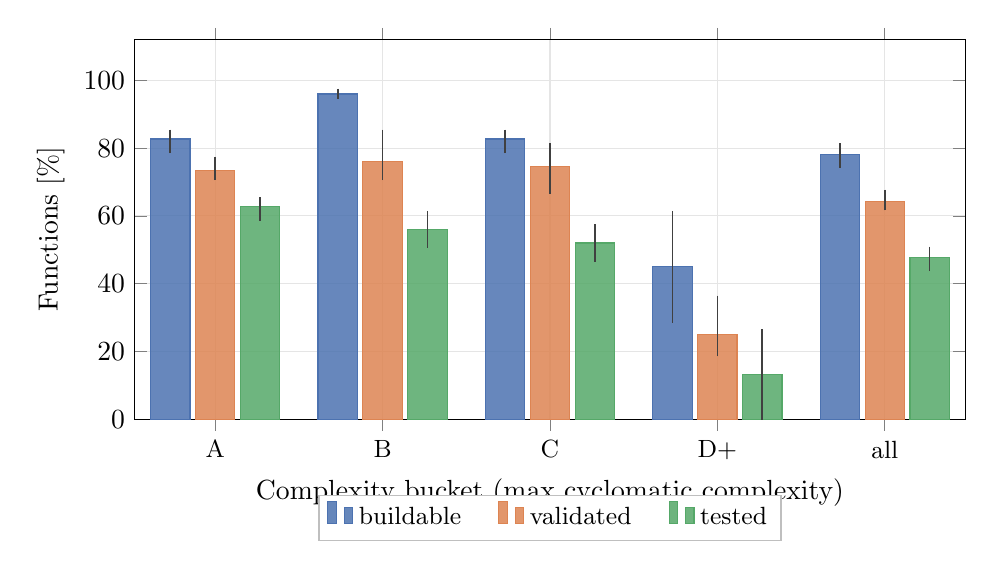
\begin{tikzpicture}
\definecolor{buildable}{HTML}{4c72b0}
\definecolor{validated}{HTML}{dd8452}
\definecolor{tested}{HTML}{55a868}
\begin{axis}[
  ybar,
  width=\linewidth, height=6.4cm,
  bar width=0.5cm,
  enlarge x limits=0.12,
  ymin=0, ymax=112,
  ytick={0,20,40,60,80,100},
  ylabel={Functions [\%]},
  xlabel={Complexity bucket (max cyclomatic complexity)},
  symbolic x coords={A,B,C,Dplus,all},
  xtick=data, xticklabels={A,B,C,D+,all},
  x tick label style={font=\small},
  grid=major, grid style={draw=black!10},
  error bars/y dir=both, error bars/y explicit,
  error bars/error bar style={black!75, line width=0.6pt},
  error bars/error mark options={black!75, line width=0.6pt, mark size=1.8pt},
  legend style={at={(0.5,-0.20)}, anchor=north, legend columns=3,
                draw=black!25, font=\small, /tikz/every even column/.append style={column sep=0.4cm}},
]
\addplot[draw=buildable, fill=buildable, fill opacity=0.85] coordinates {(A,82.7) += (0,1.3) -= (0,2.7) (B,96.0) += (0,0.0) -= (0,0.0) (C,82.7) += (0,1.3) -= (0,2.7) (Dplus,45.0) += (0,15.0) -= (0,15.0) (all,78.2) += (0,1.8) -= (0,2.5)};
\addplot[draw=validated, fill=validated, fill opacity=0.85] coordinates {(A,73.3) += (0,2.7) -= (0,1.3) (B,76.0) += (0,8.0) -= (0,4.0) (C,74.7) += (0,5.3) -= (0,6.7) (Dplus,25.0) += (0,10.0) -= (0,5.0) (all,64.2) += (0,2.1) -= (0,1.1)};
\addplot[draw=tested,    fill=tested,    fill opacity=0.85] coordinates {(A,62.7) += (0,1.3) -= (0,2.7) (B,56.0) += (0,4.0) -= (0,4.0) (C,52.0) += (0,4.0) -= (0,4.0) (Dplus,13.3) += (0,11.7) -= (0,13.3) (all,47.7) += (0,1.8) -= (0,2.5)};
\legend{buildable, validated, tested}
\end{axis}
\end{tikzpicture}

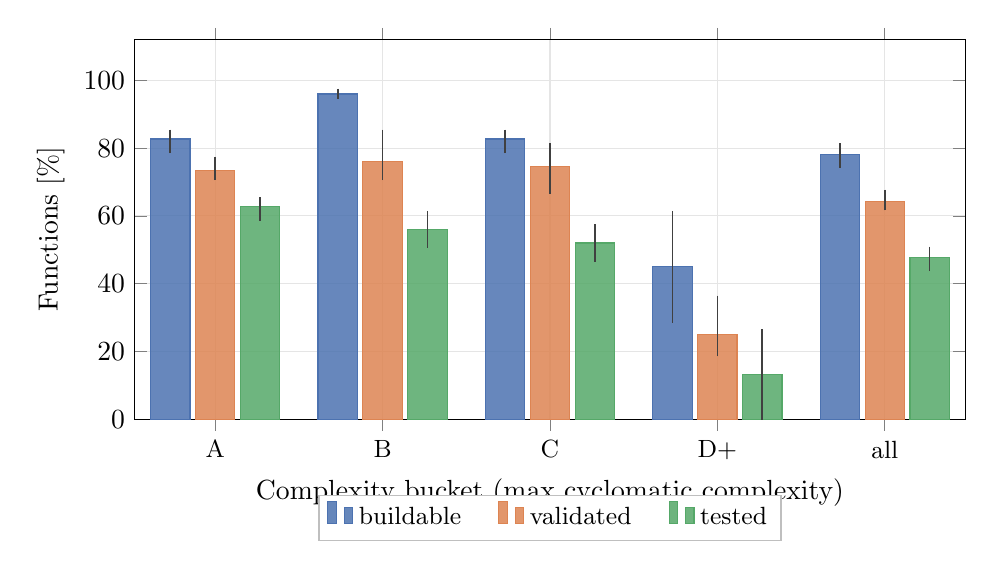
\begin{tikzpicture}
\definecolor{buildable}{HTML}{4c72b0}
\definecolor{validated}{HTML}{dd8452}
\definecolor{tested}{HTML}{55a868}
\begin{axis}[
  ybar,
  width=\linewidth, height=6.4cm,
  bar width=0.5cm,
  enlarge x limits=0.12,
  ymin=0, ymax=112,
  ytick={0,20,40,60,80,100},
  ylabel={Functions [\%]},
  xlabel={Complexity bucket (max cyclomatic complexity)},
  symbolic x coords={A,B,C,Dplus,all},
  xtick=data, xticklabels={A,B,C,D+,all},
  x tick label style={font=\small},
  grid=major, grid style={draw=black!10},
  error bars/y dir=both, error bars/y explicit,
  error bars/error bar style={black!75, line width=0.6pt},
  error bars/error mark options={black!75, line width=0.6pt, mark size=1.8pt},
  legend style={at={(0.5,-0.20)}, anchor=north, legend columns=3,
                draw=black!25, font=\small, /tikz/every even column/.append style={column sep=0.4cm}},
]
\addplot[draw=buildable, fill=buildable, fill opacity=0.85] coordinates {(A,82.7) += (0,1.3) -= (0,2.7) (B,96.0) += (0,0.0) -= (0,0.0) (C,82.7) += (0,1.3) -= (0,2.7) (Dplus,45.0) += (0,15.0) -= (0,15.0) (all,78.2) += (0,1.8) -= (0,2.5)};
\addplot[draw=validated, fill=validated, fill opacity=0.85] coordinates {(A,73.3) += (0,2.7) -= (0,1.3) (B,76.0) += (0,8.0) -= (0,4.0) (C,74.7) += (0,5.3) -= (0,6.7) (Dplus,25.0) += (0,10.0) -= (0,5.0) (all,64.2) += (0,2.1) -= (0,1.1)};
\addplot[draw=tested,    fill=tested,    fill opacity=0.85] coordinates {(A,62.7) += (0,1.3) -= (0,2.7) (B,56.0) += (0,4.0) -= (0,4.0) (C,52.0) += (0,4.0) -= (0,4.0) (Dplus,13.3) += (0,11.7) -= (0,13.3) (all,47.7) += (0,1.8) -= (0,2.5)};
\legend{buildable, validated, tested}
\end{axis}
\end{tikzpicture}

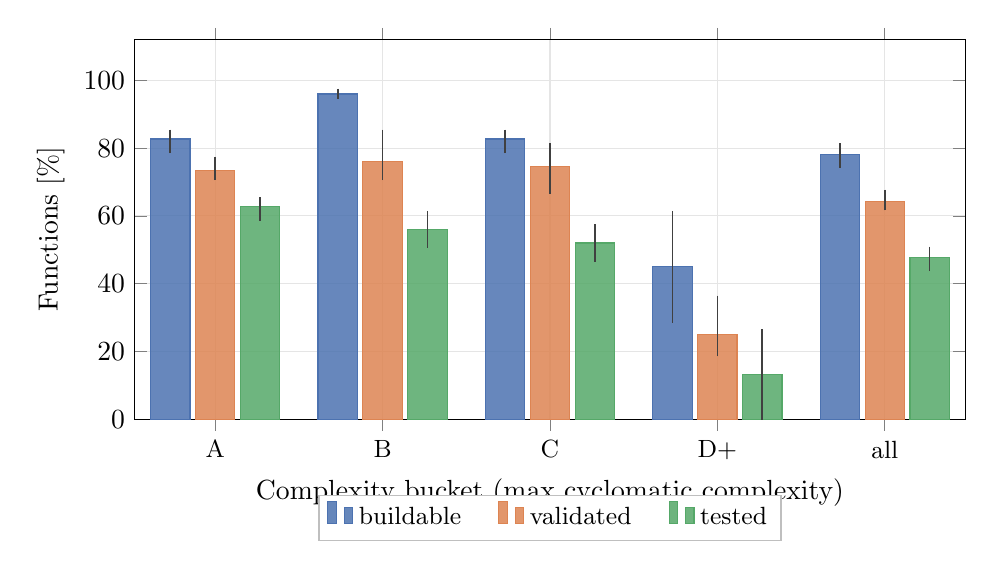
\begin{tikzpicture}
\definecolor{buildable}{HTML}{4c72b0}
\definecolor{validated}{HTML}{dd8452}
\definecolor{tested}{HTML}{55a868}
\begin{axis}[
  ybar,
  width=\linewidth, height=6.4cm,
  bar width=0.5cm,
  enlarge x limits=0.12,
  ymin=0, ymax=112,
  ytick={0,20,40,60,80,100},
  ylabel={Functions [\%]},
  xlabel={Complexity bucket (max cyclomatic complexity)},
  symbolic x coords={A,B,C,Dplus,all},
  xtick=data, xticklabels={A,B,C,D+,all},
  x tick label style={font=\small},
  grid=major, grid style={draw=black!10},
  error bars/y dir=both, error bars/y explicit,
  error bars/error bar style={black!75, line width=0.6pt},
  error bars/error mark options={black!75, line width=0.6pt, mark size=1.8pt},
  legend style={at={(0.5,-0.20)}, anchor=north, legend columns=3,
                draw=black!25, font=\small, /tikz/every even column/.append style={column sep=0.4cm}},
]
\addplot[draw=buildable, fill=buildable, fill opacity=0.85] coordinates {(A,82.7) += (0,1.3) -= (0,2.7) (B,96.0) += (0,0.0) -= (0,0.0) (C,82.7) += (0,1.3) -= (0,2.7) (Dplus,45.0) += (0,15.0) -= (0,15.0) (all,78.2) += (0,1.8) -= (0,2.5)};
\addplot[draw=validated, fill=validated, fill opacity=0.85] coordinates {(A,73.3) += (0,2.7) -= (0,1.3) (B,76.0) += (0,8.0) -= (0,4.0) (C,74.7) += (0,5.3) -= (0,6.7) (Dplus,25.0) += (0,10.0) -= (0,5.0) (all,64.2) += (0,2.1) -= (0,1.1)};
\addplot[draw=tested,    fill=tested,    fill opacity=0.85] coordinates {(A,62.7) += (0,1.3) -= (0,2.7) (B,56.0) += (0,4.0) -= (0,4.0) (C,52.0) += (0,4.0) -= (0,4.0) (Dplus,13.3) += (0,11.7) -= (0,13.3) (all,47.7) += (0,1.8) -= (0,2.5)};
\legend{buildable, validated, tested}
\end{axis}
\end{tikzpicture}

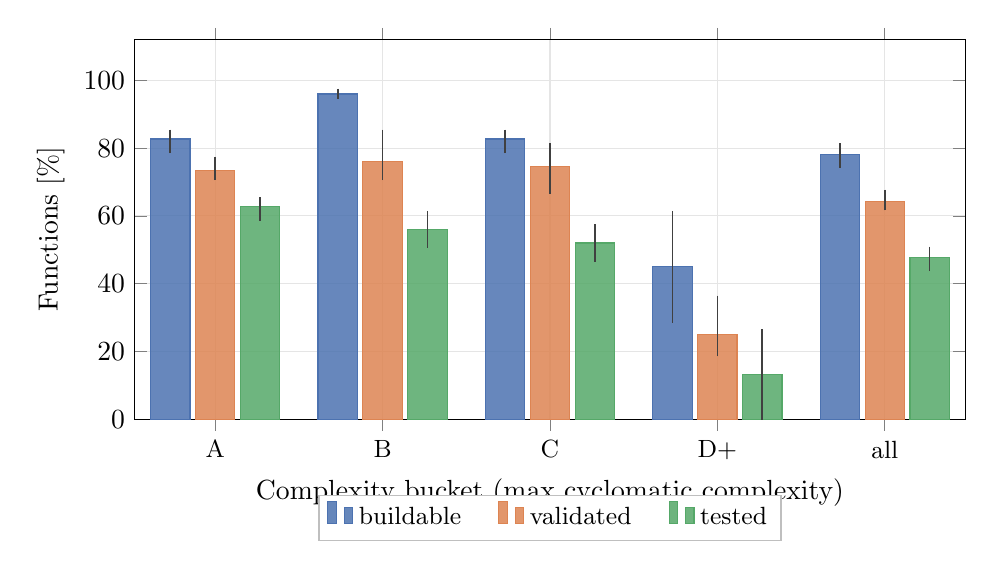
\begin{tikzpicture}
\definecolor{buildable}{HTML}{4c72b0}
\definecolor{validated}{HTML}{dd8452}
\definecolor{tested}{HTML}{55a868}
\begin{axis}[
  ybar,
  width=\linewidth, height=6.4cm,
  bar width=0.5cm,
  enlarge x limits=0.12,
  ymin=0, ymax=112,
  ytick={0,20,40,60,80,100},
  ylabel={Functions [\%]},
  xlabel={Complexity bucket (max cyclomatic complexity)},
  symbolic x coords={A,B,C,Dplus,all},
  xtick=data, xticklabels={A,B,C,D+,all},
  x tick label style={font=\small},
  grid=major, grid style={draw=black!10},
  error bars/y dir=both, error bars/y explicit,
  error bars/error bar style={black!75, line width=0.6pt},
  error bars/error mark options={black!75, line width=0.6pt, mark size=1.8pt},
  legend style={at={(0.5,-0.20)}, anchor=north, legend columns=3,
                draw=black!25, font=\small, /tikz/every even column/.append style={column sep=0.4cm}},
]
\addplot[draw=buildable, fill=buildable, fill opacity=0.85] coordinates {(A,82.7) += (0,1.3) -= (0,2.7) (B,96.0) += (0,0.0) -= (0,0.0) (C,82.7) += (0,1.3) -= (0,2.7) (Dplus,45.0) += (0,15.0) -= (0,15.0) (all,78.2) += (0,1.8) -= (0,2.5)};
\addplot[draw=validated, fill=validated, fill opacity=0.85] coordinates {(A,73.3) += (0,2.7) -= (0,1.3) (B,76.0) += (0,8.0) -= (0,4.0) (C,74.7) += (0,5.3) -= (0,6.7) (Dplus,25.0) += (0,10.0) -= (0,5.0) (all,64.2) += (0,2.1) -= (0,1.1)};
\addplot[draw=tested,    fill=tested,    fill opacity=0.85] coordinates {(A,62.7) += (0,1.3) -= (0,2.7) (B,56.0) += (0,4.0) -= (0,4.0) (C,52.0) += (0,4.0) -= (0,4.0) (Dplus,13.3) += (0,11.7) -= (0,13.3) (all,47.7) += (0,1.8) -= (0,2.5)};
\legend{buildable, validated, tested}
\end{axis}
\end{tikzpicture}
